\documentclass[12pt]{article}
\usepackage{amsmath}
\usepackage{mathdots}
\usepackage{amsthm}
\usepackage{bbold}
\usepackage{graphicx}
\title{The GHOST permutation and multi-scale resampling}
\author{Guillaume Filion}
\date{}

\newtheorem{basictheorem}{Theorem}
\newtheorem{definition}{Definition}

\begin{document}
  \maketitle

  \section{Preliminary remarks}

  Let's assume that $X = (x_1, ..., x_N)$ is a sample of size
  $N$ from a time-series. Because we can always subtract the
  mean, we will assume that $X$ has zero average without
  loss of generality.

  In what follows, we will refer to the `diagonals' of a square
  matrix as the elements of index $(i,j)$ such that $i-j$ is
  constant. An $N \times N$ matrix has $2N-1$ diagonals. We index
  them from the bottom-left to the top-right corner. The $N^{th}$
  diagonal has $N$ elements (it is `the' diagonal of a square matrix),
  whereas the $1^{st}$ and the $(2N-1)^{th}$ have only one element.
  We will occasionally use the terms `main diagonal' for $N^{th}$
  diagonal and `anti-diagonal', which means the ascending diagonal
  from left to right, or those elements of index $(i,j)$ such that
  $i+j=N+1$.

  \section{Auto-covariance and permutation matrices}

  With our convention that  $X$ has zero average throughout,
  the auto-covariance at lag $L$ of an observed time series $X$ is
  defined as $\sum_{i=1}^{N-L}x_i x_{i+L}/(N-L)$. If $X$ is stationary,
  the expected value of $x_i x_{i+L}$ is a function of $L$ only,
  a quantity that we will denote $S_X(L)$. In that case, the expected
  auto-covariance at lag $L$ of the time series is also equal to
  $S_X(L)$.

  We will consider the $N \times N$ symmetric matrix $XX^\mathsf{T}$,
  whose element of index $(i,j)$ is $x_i x_j$. The mean of the
  $(N+L)^{th}$ --- or $(N-L)^{th}$ --- diagonal of $XX^\mathsf{T}$ is by
  definition the auto-covariance of $X$ at lag $L$. This is why 
  we will refer to $XX^\mathsf{T}$ as the auto-covariance matrix
  of $X$.

  If $X$ is sampled from a stationary time series, $E\{XX^\mathsf{T}\}$
  contains at most $N$ distinct values, and the values along diagonals
  are identical. In that case, the expected auto-covariance matrix
  is said to have a `Toeplitz structure' (here $E$ represents the
  expectation taken from the distribution of the random variable $X$).
  More specifically,

  \begin{equation}
    E\{X X^\mathsf{T}\} = \left( \begin{array}{ccccc}
      S_X(0) & S_X(1) & S_X(2) & \ldots & S_X(N) \\
      S_X(1) & S_X(0) & S_X(1) & \ldots & S_X(N-1) \\
      S_X(2) & S_X(1) & S_X(0) & \ldots & S_X(N-2) \\
      \vdots & \vdots & \vdots & \ddots & \vdots \\
      S_X(N) & S_X(N-1) & S_X(N-2) & \ldots & S_X(0)
    \end{array}
    \right).
  \end{equation}

  Any permutation of the time series $X$ can be described
  by an $N \times N$ matrix of 0's and 1's such that there is
  exactly one 1 per column and per row. The matrix associated
  to a permutation $\sigma$ will be denoted $M_\sigma$. The presence
  of a 1 at index $(i,j)$ means $\sigma(i)=j$. It follows from this
  observation that $M_\sigma^{\mathsf{T}}$ is the inverse of 
  $M_\sigma$ and that $\sigma$ is an orthogonal operator.

  Below is an example of a permutation $\sigma$ that transposes
  the first and third elements of a series of length 4:
 
  \begin{equation*}
    \sigma(X) = M_{\sigma} X =
    \left(
    \begin{array}{cccc}
      0 & 0 & 1 & 0 \\
      0 & 1 & 0 & 0 \\
      1 & 0 & 0 & 0 \\
      0 & 0 & 0 & 1
    \end{array}
    \right)
    \left(
    \begin{array}{c}
      x_1 \\
      x_2 \\
      x_3 \\
      x_4
    \end{array}
    \right) =
    \left(
    \begin{array}{c}
      x_3 \\
      x_2 \\
      x_1 \\
      x_4
    \end{array}
    \right).
  \end{equation*}

  The auto-covariance matrix of a series $X$ permuted by $\sigma$
  is $M_\sigma XX^\mathsf{T} M_\sigma^\mathsf{T}$
  and for fixed $\sigma$, the expected auto-covariance matrix is
  $M_\sigma E\{XX^\mathsf{T}\} M_\sigma^\mathsf{T}$.
  In general, only the elements of the main diagonal of the expected 
  auto-covariance matrix will remain identical. For a stationary
  signal of length 4, the previous example yields:

  \begin{equation*}
    M_\sigma E\{XX^\mathsf{T}\} M_\sigma^\mathsf{T} =
    \left(
    \begin{array}{cccc}
      S_X(0) & S_X(1) & S_X(2) & S_X(1) \\
      S_X(1) & S_X(0) & S_X(1) & S_X(2) \\
      S_X(2) & S_X(1) & S_X(0) & S_X(3) \\
      S_X(1) & S_X(2) & S_X(3) & S_X(0) \\
    \end{array}
    \right)
  \end{equation*}

  The fact that this matrix does not have a Toeplitz structure shows that
  permutations of a stationary signal are in general not stationary.
  However, the auto-covariance is still defined in the same way,
  so that the auto-covariance of a permuted series at lag $L$ can
  still be computed by averaging the terms of the $(N+L)^{th}$
  diagonal.

  \section{GHOST permutations and matrices}

  In what follows, $N = 2^n$ for some $n \in \mathbb{N}$.

  \begin{definition}

    The group of GHOST permutations of order $n$ is the group of
    permutations generated by permutations $\sigma$ such that there
    exists integers $k \geq 0$ and $m \geq 1$ such that $\sigma$ is an
    inversion of the elements of indices comprised between $k2^m + 1$
    and $(k+1)2^m$.
  
  \end{definition}

  For $N = 8$, $(2,1,3,4,5,6,7,8)$ and $(1,2,3,4,8,7,6,5)$ are in the
  generator, but $(1,3,2,4,5,6,7,8)$ and $(1,2,6,5,4,3,7,9)$ are not.
  The matrix representation of those example inversions is (leaving out
  the 0's for contrast):

  \begin{equation*}
    \left( \begin{array}{cccccccc}
        & 1 & & & & & & \\
        1 & & & & & & & \\
        & & 1 & & & & & \\
        & & & 1 & & & & \\
        & & & & 1 & & & \\
        & & & & & 1 & & \\
        & & & & & & 1 & \\
        & & & & & & & 1
    \end{array}
    \right) \text{, and }
    \left( \begin{array}{cccccccc}
        1 & & & & & & & \\
        & 1 & & & & & & \\
        & & 1 & & & & & \\
        & & & 1 & & & & \\
        & & & & & & & 1 \\
        & & & & & & 1 & \\
        & & & & & 1 & & \\
        & & & & 1 & & & 
    \end{array}
    \right).
  \end{equation*}

  It follows from the definition that every matrix of a GHOST
  permutation can be written as the product of $n$ diagonal block
  matrices with block sizes $2^m, (m = 1, ..., n)$. The blocks consist
  of 1's along the main diagonal or the anti-diagonal. Matrices
  of a GHOST permutations will be called `GHOST matrices'.

  For every $2^n \times 2^n$ matrix $G$, $G^{\mathsf{T}}$ =
  $\bar{I}_nG\bar{I}_n$, where $\bar{I}_n$ is ithe $2^n \times 2^n$
  matrix with 1's along the anti-diagonal and 0 everywhere else.
  $\bar{I}_n$ is a GHOST matrix because it belongs to the generator
  (for $k=0$ and $m=n$), which shows that the transpose of a GHOST
  matrix is also a GHOST matrix.

  \section{Random GHOST permutations}

  A level $m$ GHOST matrix consists of $2^n / 2^m = 2^{n-m}$ blocks,
  each of which can be in 2 states, so there are $2^{2^{n-m}}$
  such matrices. Every GHOST matrix is the  product of $n$ level
  $m, (m=1, ..., n)$ GHOST matrices so the total number of GHOST
  matrices is $2^{2^n - 1} = 2^{N-1}$. Even though this number
  scales exponentially with the series length $N$, it constitutes
  a tiny fraction of $N!$, the total number of permutations of $X$.

  We will assume a uniform probability measure on the set of GHOST
  permutations. The decomposition of GHOST matrices in level
  $m, (m = 1, ..., n)$ GHOST matrices gives a method to generate
  GHOST permutations at random: one simply inverts the blocks showed
  by this decomposition with probability 1/2.

  \begin{basictheorem}\label{uniformity}
    $E\{ M_\sigma \} = \frac{1}{2^n} \mathbb{1}$ 
    where $\mathbb{1}$ is the $2^n \times 2^n$
    matrix filled with 1's, and $E$ is the expectation with respect to
    the uniform probability measure on GHOST permutations.
  \end{basictheorem}

  \begin{proof}
    We proceed by induction on $n$. For $n=1$ we have
    \begin{equation*}
      E\{ M_\sigma \} =
      \frac{1}{2} \left( \begin{array}{cc}
        1 & 0 \\
        0 & 1
      \end{array} \right) +
      \frac{1}{2} \left( \begin{array}{cc}
        0 & 1 \\
        1 & 0
      \end{array} \right) =
      \frac{1}{2} \left( \begin{array}{cc}
        1 & 1 \\
        1 & 1
      \end{array} \right).
    \end{equation*}

    Now assume that the result has been proven at rank $n$.
    Every GHOST matrix of order $n+1$ can be expressed as 
    a block matrix with 2 blocks of size $2^n$, each of which is
    a GHOST matrix of order $n$, \textit{i.e.}

    \begin{equation*}
      \left( \begin{array}{cc}
        G_1 & 0 \\
        0   & G_2
      \end{array} \right) \text{ or }
      \left( \begin{array}{cc}
        0 & G_3 \\
        G_4 & 0
      \end{array} \right),
    \end{equation*}

    \noindent
    with equal probability, where $G_1$ and $G_2$ are GHOST matrices
    of order $n$. Using the induction hypothesis, it comes: 

    \begin{equation*}
      E\{ M_\sigma \} = 
      \frac{1}{2} \left( \begin{array}{cc}
        E\{ G_1 \} & 0 \\
        0   & E \{ G_2 \}
      \end{array} \right) +
      \frac{1}{2} \left( \begin{array}{cc}
        0 & E \{ G_3 \} \\
        E \{ G_4 \} & 0
      \end{array} \right) = \frac{1}{2^{n+1}} \mathbb{1}.
    \end{equation*}

  \end{proof}

  In other terms, upon applying a random GHOST permutation to a
  sample, every element has equal chances of replacing any other
  element. However, in GHOST permutations the placement of an element
  is not independent of the placement of others, as we will see now.

  \section{GHOST auto-covariance}

  Let $X$ be a sample of size $N = 2^n$ from a stationary time series.
  We denote $A = E\{XX^\mathsf{T}\}$ the expected auto-covariance matrix
  of $X$ under the expectation taken from the distribution of $X$.
  To compute the quantity $E\{M_\sigma A M_\sigma^\mathsf{T}\}$,
  where the expectation is taken over the GHOST permutations
  $\sigma$, we introduce the following term:

  \begin{definition}\label{kblocks}
    A $k$-block of a $2^n \times 2^n$ matrix is a $2^k \times 2^k$ block
    such that there exists integers $k \geq0$ and $m \geq 1$ such that
    the top-left corner of the block has coordinates
    $(2k2^m+1, (2k+1)2^m+1)$ or $((2k+1)2^m+1, 2k2^m+1)$.
  \end{definition}

  The decomposition of a  $2^n \times 2^n$ matrix in
  $k$-blocks, $(k=0, ..., n-1)$ is unique. A $2 \times 2$ matrix
  comprises two diagonal terms and two 0-blocks, A $4 \times 4$ matrix
  comprises four diagonal terms, four 0-blocks and two 1-blocks
  \textit{etc}. The following example enhances the decomposition
  of an $8 \times 8$ matrix in $k$-blocks. Elements of a $k$-block
  are labelled with number $k$:

  \begin{equation*}
    \left( \begin{array}{cccccccc}
       & 0 & 1 & 1 & 2 & 2 & 2 & 2 \\
      0 &  & 1 & 1 & 2 & 2 & 2 & 2 \\
      1 & 1 &  & 0 & 2 & 2 & 2 & 2 \\
      1 & 1 & 0 &  & 2 & 2 & 2 & 2 \\
      2 & 2 & 2 & 2 &  & 0 & 1 & 1  \\
      2 & 2 & 2 & 2 & 0 &  & 1 & 1  \\
      2 & 2 & 2 & 2 & 1 & 1 &  & 0  \\
      2 & 2 & 2 & 2 & 1 & 1 & 0 &  
    \end{array} \right)
  \end{equation*}

  \begin{basictheorem}\label{acmatrix}
    $E\{M_\sigma A M_\sigma^\mathsf{T}\}$ has a structure in $k$-blocks,
    where the elements of a $k$-block are all equal to the average of
    elements of a $k$-block of $A$ and the diagonal elements are the
    same as those of $A$.
  \end{basictheorem}

  \begin{proof}

  First, notice that because $A$ has a symmetric Toeplitz structure,
  all its $k$-blocks are identical. Thus, taking the average of
  of the elements of any $k$-block gives the same value.

  As in theorem \ref{uniformity}, we proceed by induction on $n$.
  For $n = 1$,

  \begin{eqnarray*}
    E\{M_\sigma A M_\sigma^\mathsf{T}\} = 
    &\,& \frac{1}{2} \left( \begin{array}{cc}
      S_X(0) & S_X(1) \\
      S_X(1) & S_X(0)
    \end{array} \right) + \\
    &\,& \frac{1}{2} \left( \begin{array}{cc}
      S_X(0) & S_X(1) \\
      S_X(1) & S_X(0)
    \end{array} \right) = 
    \left( \begin{array}{cc}
      S_X(0) & S_X(1) \\
      S_X(1) & S_X(0)
    \end{array} \right).
  \end{eqnarray*}

  This matrix trivially has the announced properties.
  Suppose now that the formula is proven at rank $n$.
  Let us decompose the matrix $A$ in blocks of
  size $2^n$. Because of its Toeplitz and symmetric structure,
  the diagonal and anti-diagonal blocs are identical. We denote
  them $A_1$ and $A_2$, respectively. Like in the proof of 
  theorem \ref{uniformity}, there are two equiprobable
  decompositions of a random GHOST matrix of order $n+1$.

  \begin{align}
    E\{M_\sigma A M_\sigma^\mathsf{T}\} =
    \frac{1}{2} E \left\{
    \left( \begin{array}{cc}
      G_1 & 0 \\
      0   & G_2
    \end{array} \right)
    \left( \begin{array}{cc}
      A_1 & A_2 \\
      A_2 & A_1
    \end{array} \right)
    \left( \begin{array}{cc}
      G_1^\mathsf{T} & 0 \\
      0  & G_2^\mathsf{T}
    \end{array} \right) \right\} + \notag \\
    \frac{1}{2} E \left\{
    \left( \begin{array}{cc}
      0 & G_3\\
      G_4 & 0
    \end{array} \right)
    \left( \begin{array}{cc}
      A_1 & A_2 \\
      A_2 & A_1
    \end{array} \right)
    \left( \begin{array}{cc}
      0 & G_4^\mathsf{T} \\
      G_3^\mathsf{T} & 0
    \end{array} \right) \right\} = \quad \\
    \frac{1}{2} \left( \begin{array}{cc}
      E\{G_1 A_1 G_1^\mathsf{T}\} + E\{G_3 A_1 G_3^\mathsf{T}\}
        & E\{G_1 A_2 G_2^\mathsf{T}\} + E\{G_3 A_2 G_4^\mathsf{T}\}\\
      E\{G_2 A_2 G_1^\mathsf{T}\} + E\{G_4 A_2 G_3^\mathsf{T}\}
        & E\{G_2 A_1 G_2^\mathsf{T}\} + E\{G_4 A_1 G_4^\mathsf{T}\}
    \end{array} \right). \notag
  \end{align}

  Matrices $G$ with a different index are sampled independently,
  so the off-diagonal terms reduce to
  $\mathbb{1}A_2\mathbb{1}/2^{2n} = \langle A_2\rangle\mathbb{1}$,
  by theorem \ref{uniformity}, where $\langle A_2 \rangle$ is the
  mean of the $2^{2n}$ terms of $A_2$. Notice that $A_2$ is an
  $n$-block of $A$. Using the induction hypothesis we get

  \begin{equation*}
    E\{M_\sigma A M_\sigma^\mathsf{T}\} =
    \left( \begin{array}{cc}
      * & \langle A_2\rangle\mathbb{1} \\
      \langle A_2\rangle\mathbb{1} & *
    \end{array} \right),
  \end{equation*}

  \noindent
  where $*$ designates the matrix with a structure in $k$-blocks
  obtained from the induction hypothesis. But this matrix has a
  structure in $k$-blocks with the announced value.

  \end{proof}

  This allows us to compute the auto-covariance of a GHOST-permuted
  stationary signal at any lag.

  \begin{basictheorem}\label{acf}
    Let $X$ be a stationary time series of length $2^n$ and $Y$ obtained
    by applying a random GHOST permutation on $X$.
    The expected auto-covariance of $Y$ is
      \begin{eqnarray}
        E\{S_Y(L)\} = 
        \frac{2^{n-1}}{2^n-L}\sum_{k=0}^{n-1} \frac{\varphi_{2^k}(L)}{8^k}
          \sum_{l=1}^{2^{k+1}-1} \varphi_{2^k}(l) S_X(l)
          \label{acfL} \text{, where} \\
        \varphi_{2^k}(l) = \left\{
          \begin{array}{cc}
            l & \text{ if } 0 < l \leq 2^k, \\
            2^{k+1}-l & \text{ if } 2^k < l \leq 2^{k+1}, \\
            0 & \text{ otherwise.}
          \end{array}
          \right. \label{phi}
      \end{eqnarray}
       
  \end{basictheorem}

  Note that GHOST-permuted signals are not stationary.

  Intuitively $\varphi_{2^k}(l)$ can be viewed as the number of elements
  along the $l^{th}$ diagonal of a $2^k \times 2^k$ matrix.
  $\varphi_{2^k}(l)$ increases from 1 to $2^k$ (the main diagonal) and
  then decreases to 1 as $l$ ranges from 1 to $2^{2k}-1$.

  \begin{proof}[Proof of theorem \ref{acf}]
    For any signal $Y$ of length $N$, the auto-covariance at lag $L$
    is given by averaging the terms along the $(N+L)^{th}$ diagonal of
    $E\{YY^{\mathsf{T}}\}$. Here $N = 2^n$ and $E\{YY^{\mathsf{T}}\}$
    has a structure in $k$-blocks according to theorem \ref{acmatrix}.
    We proceed by counting the $k$-blocks crossed by the $(2^n+L)^{th}$
    diagonal and counting the portion of the diagonal that lies in
    each $k$-block.

    Definition \ref{kblocks} shows that there are $2^n/2^k = 2^{n-k}$
    $k$-blocks, \textit{i.e.} $2^{n-k-1}$ on the right side of the
    diagonal. For a given $k$-block, the number of elements belonging
    to the $(2^n+L)^{th}$ diagonal is $\varphi_{2^k}(L)$ according
    to our interpretation of $\varphi_{2^k}$ (the bottom-left corner
    of every $k$-block is along the $(2^n+1)^{th}$ diagonal). So the total
    number of elements of the $(2^n+L)^{th}$ diagonal in any $k$-block is
    $2^{n-k-1}\varphi_{2^k}(L)$.

    The elements of a $k$-block of $E\{YY^{\mathsf{T}}\}$ are identical,
    and their value can be computed by theorem \ref{acmatrix}.
    The $k$-blocks of $A = E\{XX^{\mathsf{T}}\}$ contain values
    $S_X(l), (l=1, ..., 2^{k+1}-1)$. Because $A$ has a symmetric Teoplitz
    structure, the value $S_X(l)$ is present $\varphi_{2^k}(l)$ times
    per $k$-block, so the average is

    \begin{equation*}
      \sum_{l=1}^{2^{k+1}-1} \varphi_{2^k}(l) S_X(l) / 2^{2k}.
    \end{equation*}

    Combining these two results, summing over $k$ and keeping in mind
    that the $(2^n+L)^{th}$ diagonal of $E\{YY^{\mathsf{T}}\}$ has
    $2^n-L$ elements gives formula (\ref{acfL}).

  \end{proof}

  In other words, the expected auto-covariance of a GHOST-permuted
  stationary signal is a linear transformation of the expected
  auto-covariance of the original signal. 

  \begin{definition}\label{R}
    We will call $R_{2^n-1}$ the $(2^n-1) \times (2^n-1)$ matrix whose
    element of index $(i,j)$ is
    \begin{equation}
      \label{matrixelements}
        \frac{2^{n-1}}{2^n-i}\sum_{k=0}^{n-1}
          \frac{\varphi_{2^k}(i)\varphi_{2^k}(j)}{8^k}
    \end{equation}

  \end{definition}

  By definition, the lines of $R_{2^n-1}$ are the weights
  of formula (\ref{acfL}). If $S_X$ is the vector of expected
  auto-covariance terms of a stationary signal $X$ at lags
  $1, 2, ..., 2^n-1$, then the expected auto-covariance terms of the
  GHOST-permuted signal are given by $R_{2^n-1} S_X$.
  The left panel of figure \ref{matrices} gives a representation of
  $R_{15}$, the linear operator that gives the expected auto-covariance
  of a GHOST-permuted signal of length 16. The diagonal becomes
  progressively blurred: as the lag increases, the weights become
  more uniform.

  Permutation of a signal does not change its variance, which is the
  auto-covariance term at lag $L=0$. $R_{2^n-1}$ can be extended to a
  $2^n \times 2^n$ matrix $\tilde{R}_{2^n}$ that maps the
  full auto-covariance series, by adding a row at the top and a column
  at the left consisting of 1 at position $(1,1)$ and 0 everywhere
  else as shown in the right panel of figure \ref{matrices}. In this
  matrix, the auto-covariance term at lag $L$ is given by row $L+1$.

  % R matrices figure. %
  \begin{figure}[t] 
  \centering
  
\includegraphics{matrices_GF110823.pdf}
  \caption{Graphical representation of $R_{15}$ and $\tilde{R}_{16}$.
  Left panel: the linear operator $R_{15}$ maps the expected
  auto-covariance of a signal of length 16 to the expected
  auto-covariance of the GHOST-permuted signal. Right panel: the linear
  operator $\tilde{R}_{16}$ maps the full auto-covariance (including
  the variance term).
  The intensity of the gray squares is proportional to the value of
  the corresponding element (0 is white and 1 is black).}
  \label{matrices}
  \end{figure}

  % Stochastic matrices. %
  \begin{basictheorem}\label{stochastic}
    For every $n \geq 1$, $R_{2^n-1}$ and $\tilde{R}_{2^n}$ are
    stochastic matrices (all their elements are positive real, and their
    rows add up to 1). In addition, the bottom $2^{n-1}$ rows of
    $R_{2^n-1}$ (and thus $\tilde{R}_{2^n}$) are identical.
  \end{basictheorem}

  \begin{proof}
    The elements of $R_{2^n-1}$ are obviously positive real. To compute
    the row-wise sum, observe that for every $k \geq 1$

    \begin{equation*}
      \sum_{j=1}^{2^n-1}\varphi_{2^k}(j) = 
        2(1+2+...+2^k-1) + 2^k = 2^{2k} = 4^k,
    \end{equation*}

  \noindent
  so that the value of the sum is
    
    \begin{equation}\label{sum}
      S(i) = \frac{2^{n-1}}{2^n-i}\sum_{k=0}^{n-1}\varphi_{2^k}(i)/2^k.
    \end{equation}

  For every $i < 2^n$, there exists a unique $m$ such that
  $2^{m-1} < i \leq 2^m$. Now

  \begin{equation*}
    \varphi_{2^k}(i) = \left\{
      \begin{array}{cc}
        0 & \text{ if } k < m-1, \\
        2^m-i & \text{ if } k = m-1, \\
        i & \text{ otherwise.}
      \end{array}
      \right. \label{phi}
  \end{equation*}

  Using this, equation (\ref{sum}) yields

  \begin{eqnarray*}
    S(i) &=& \frac{2^{n-1}}{2^n-i} \left( \frac{2^m-i}{2^{m-1}} +
        i \sum_{k=m}^{n-1}\frac{1}{2^k} \right) \\
      &=& \frac{2^{n-1}}{2^n-i} \left( \frac{2^m-i}{2^{m-1}} +
        \frac{i}{2^{m-1}} - \frac{i}{2^{n-1}} \right)
        = \frac{2^{n-1}}{2^n-i} \left(2 - \frac{i}{2^{n-1}} \right)
        = 1.
  \end{eqnarray*}

  This proves that $R_{2^n-1}$ is a stochastic matrix.
  By definition, $\tilde{R}_{2^n}$, is trivially stochastic
  if $R_{2^n-1}$ is.

  The $2^{n-1}$ bottom rows of $R_{2^n-1}$ are such that 
  $2^{n-1} \leq i \leq 2^n-1$, so $\varphi_{2^k}(i) = 0$ for
  $k \neq n-1$ and $\varphi_{2^{n-1}}(i) = 2^n -i$. Using formula
  (\ref{matrixelements}), the element of index $(i,j)$ is seen to be
  $\varphi_{2^{n-1}}(j)/4^{n-1}$, which does not depend on $i$,
  showing that all those rows are identical.

  \end{proof}

  Note that $R_{2^n-1}$ and $\tilde{R}_{2^n}$ are not symmetric
  and that their columns do not add up to 1.

  \section{Practical examples}

  Real life stationary time series typically have a decreasing
  auto-correlation. The trend can be an exponential decrease, for short
  memory processes, or power law decrease for long memory processes.

  As an example of short memory process, let's consider a 2-state
  Markov chain $Y(q)$ with transition probability $q$, \textit{i.e.}
  with the following transition matrix:

  \begin{equation*}
    Q = \left( \begin{array}{cc}
      1-q & q \\
      q & 1-q
    \end{array} \right).
  \end{equation*}

  Elementary matrix algebra shows that the probability that $Y_n(q)$
  is in the same state as $Y_{n+L}(q)$ is $1/2+(1-2q)^L/2$.
  If the states are associated with numeric values -1 and 1, the
  process has mean 0 and variance 1. The auto-correlation at lag $L$
  is thus $(1-2q)^L$, which decreases exponentially with $L$.

  Figure \ref{shortmem1} compares the auto-correlation of $Y(q)$ to that
  of its GHOSTs for different values of $q$ for a time-series of length
  $2^8=256$. The auto-correlations are qualitatively similar,
  but as $q$ decreases, the GHOST auto-correlation at large
  lags shows an obvious lack of fit.

  % Short memory figure, increasing q. %
  \begin{figure}[t] 
  \centering
  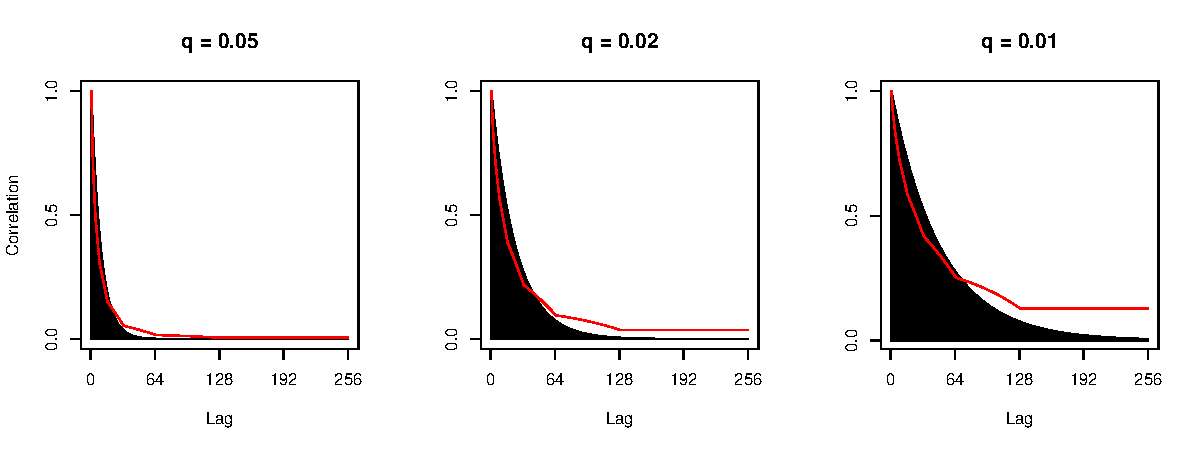
\includegraphics[scale=.7]{practical-short-mem-1_GF110907.pdf}
  \caption{Comparison of the auto-correlation of $Y(q)$ and the expected
  auto-correlation of its GHOSTs. The auto-correlation is plotted for
  a sample signal of size $2^8=256$.}
  \label{shortmem1}
  \end{figure}

  The plot also shows that the GHOST auto-correlation becomes flat
  from lag 128 onward. This is so because the rows 129 to 255 of the
  matrix $R_{2^n-1}$ are identical. This is however not the case
  as $n$ increases. As shown in figure \ref{shortmem2}, increasing
  sample size partly corrects for this lack of fit.

  % Short memory figure, increasing n. %
  \begin{figure}[t] 
  \centering
  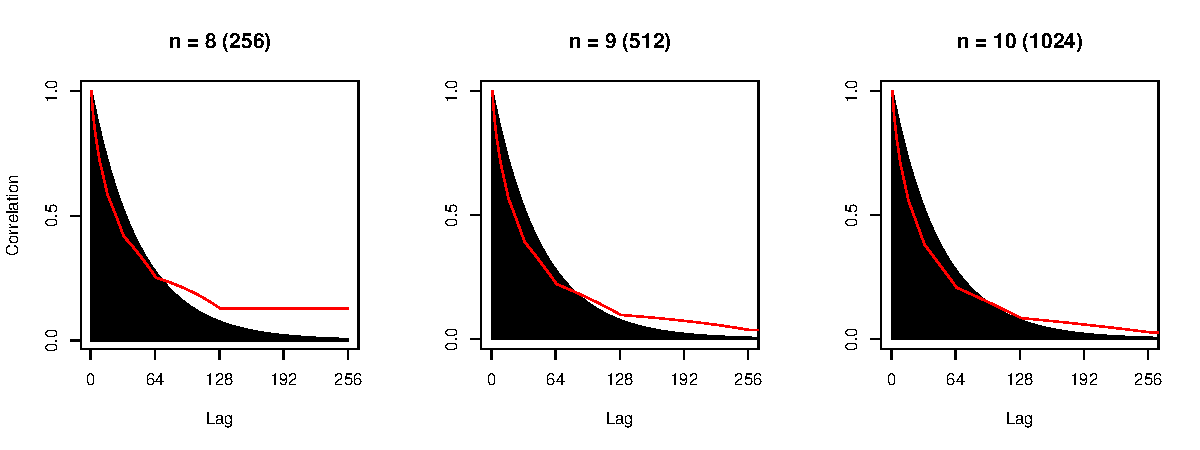
\includegraphics[scale=.7]{practical-short-mem-2_GF110907.pdf}
  \caption{Comparison of the auto-correlation of $Y(0.01)$ and the expected
  auto-correlation of its GHOSTs at different sample sizes.
  Only the auto-correlation out to lag 255 is plotted in each case.}
  \label{shortmem2}
  \end{figure}

  Let's now consider a long memory process $Z(\alpha)$ with pure power
  law, \textit{i.e.} the auto-correlation at lag $L$ is
  $(1+L)^{-\alpha}$. Figure
  \ref{longmem1} shows a comparison of the original and GHOST
  auto-covariances for different values of $\alpha$ for a sample
  of size $2^8=256$ taken from a pure power law process. Because
  of the flatness of the auto-correlation at large lags, the GHOST
  auto-covariance is a better fit in that case than for short
  memory processes.

  % Long memory figure, increasing alpha. %
  \begin{figure}[t] 
  \centering
  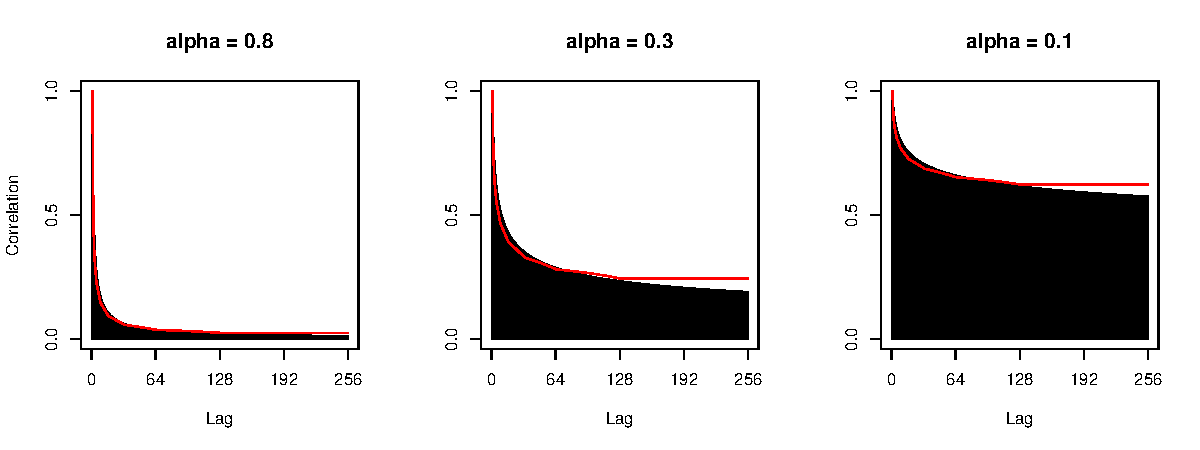
\includegraphics[scale=.7]{practical-long-mem-1_GF110907.pdf}
  \caption{Comparison of the auto-correlation of $Z(\alpha)$ and the
  expected auto-correlation of its GHOSTs for different values of
  $\alpha$. The auto-correlation is plotted for a sample size of
  $2^8=256$.}
  \label{longmem1}
  \end{figure}

  % Long memory figure, increasing n. %
  \begin{figure}[t] 
  \centering
  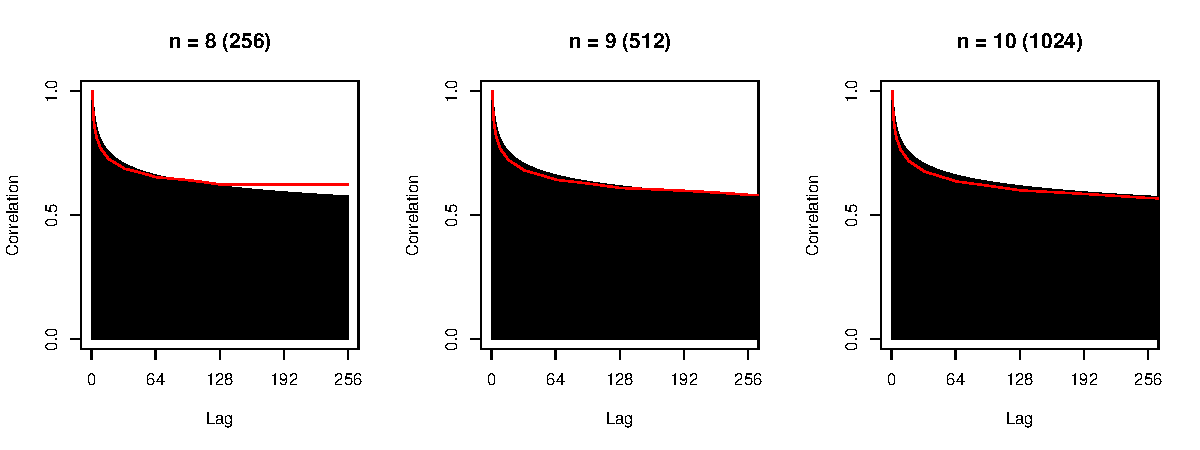
\includegraphics[scale=.7]{practical-long-mem-2_GF110907.pdf}
  \caption{Comparison of the auto-correlation of $Z(0.1)$ and the
  expected auto-correlation of its GHOSTs for different sample sizes.
  Only the auto-correlation out to lag 255 is plotted in each case.}
  \label{longmem1}
  \end{figure}

  Let us illustrate an example of GHOST permutation of a random
  signal with long memory process. We will use a fractionally
  differenced process [[refs]] because it is easy to simulate with
  the Davies-Harte method [[ref]]. The auto-covariance of a 
  fractionally differenced process $X$ with parameter $\delta$
  is given by

  \begin{equation*}
     S_X(L) = \frac{\sin(\pi\delta) \Gamma(1-2\delta) \Gamma(L +
       \delta)}{\pi \Gamma(L + 1 - \delta)}
     = O(L^{2\delta -1}).
  \end{equation*}

 
  
  The top-left panel of figure \ref{profiles} shows a sample of size
  $2^{12}=4096$ from a Gaussian fractionally differenced process with
  paramter $\delta = 0.4$ generated by the Davies-Harte method. The
  bottom-left panel is a representation of a random GHOST premutation
  of the sample. Measurements have the same color in both plots
  to easily track how the series has been shuffled.

  The right panels show the auto-covariance sequences out to lag 500.
  The auto-covariance of the GHOST drops faster, but with a similar
  trend.


  
  % Long memory figure, increasing n. %
  \begin{figure}[t] 
  \centering
  \includegraphics[scale=.52]{profiles_GF110910.pdf}
  \caption{
  Some sort of legend.
  }
  \label{profiles}
  \end{figure}


\end{document}
